\section{Conceptual diagrams}
\label{sec:diagrams}

\begin{quotation}%
Thomson: I usually write down data structures before I write down code. I don't write
algorithms --- no flowcharts, or stuff like that. But stuff you have to refer 
to on almost every line of code --- data structures.

\vspace*{1mm}

Seibel: If you're writing a C program, does that mean C code that would define those
data structures?

\vspace*{1mm}

Thomson: No, little boxes with arrows and stuff.
\\ \quotationsource \Person[Ken]{Thomson} interviewed by \textcite[p. 459]{Seibel2009}
\end{quotation}

\noindent Drawings and graphical symbols predate written language.  In contrast
to character based writing systems, a diagram can convey meaning rather
directly using elements and space as visual and spatial methaphors
\cite{Tversky2001,Winn1990}. Beside spatial data in geographic maps, however,
the use of diagrams to convey data is relatively new \cite{Tufte2001}.  Common
diagram types such as bar chart, pie chart, and line graph were developed by
\Person[William]{Playfair} (1759-1823). The focus of this thesis is data as bits
instead of data as measures and numbers. For this reason the majority of
graphical methods for statistical data, as widely used in \Term{data
visualization} \cite{Friendly2009} are not relevant to this thesis. Diagrams as
methods for data description and structuring can best be summarized as
\Term{conceptual diagrams}: an example of a conceptual diagram is an
organizational chart which represents organizational parts and their
relationships in a company.

Conceptual diagrams are popular methods especially to abstract from an universe
of discourse in the act of \term{data modeling}.  Pictoral and graphical
representations even turned out to be the most mentioned theme in a survey
among 104 data modeling practitioners, asked for a definition of data modeling
\cite[p.  192]{Simsion2007}.

Conceptual diagrams can structure and describe data but they are also a form of
data if they follow the visual \term{notation} of a diagrammatic \term{writing
system}. To justify this view we can compare diagrams with written text -- both
can be based on defined symbols (see section~\ref{sec:characters}). Once these
symbols are identified in a visual notation, the diagram or text can be
reproduced without any loss of information. A \Term{visual notation} is formed
by a set of \Term[visual symbol]{visual symbols} and a set of rules how to
combine these symbols to valid diagrams \cite{Moody2009,Costagliola2004}.  The
argument for treating conceptual diagrams as data is outlined in
appendix~\ref{appendixB}. The primary problem is a problem of digitization,
similar to \tacro{optical character recognition}{OCR} for textual data.

The following section will first list existing types of conceptual diagrams
(section~\ref{sec:diagramtypes}) and second summarize their common properties
and elements (section~\ref{sec:diagramproperties}). Diagram types for
processes, such as flow charts, business rules and visual programming languages
are not included because of the focus of this thesis on static digital documents.


\subsection{Diagram types}
\label{sec:diagramtypes}

\subsubsection{Conceptual modeling notations}

An early and influental graphical notation for data was introduced by
\textcite{Bachman1969} as \Term{data-structure diagram}, also known as
\term{Bachman diagram} . Bachman compared his diagrams with \tacro{Critical
Path Method}{CPM} and \tacro{Program Evaluation and Review Technique}{PERT}
diagrams that had been developed for project management in the late 1950s. A
simple example of a data-structure diagram is included in
figure~\ref{fig:hnetexamples}.  Based on Bachman, \textcite{Chen1976}
introduced \acro{ERM} (section~\ref{sec:erm}) together with
\term[entity-relationship diagram] {entity-relationship diagrams}. Similar
conceptual diagram types are associated with other conceptual modeling
languages such as \acro{UML} (section~\ref{sec:uml}) and \acro{ORM}
(section~\ref{sec:orm}).  Elements of these diagram types, such as notations
for entity types, attributes, roles, rules, and constraints (see
figure~\ref{fig:orm2basics}) mirror elements and constructs of their modeling
language, as listed and described at page~\pageref{ermconceptualconstructs} in
section \ref{sec:erm}. An example of visual notation variants is given in
table~\ref{tab:ermnotations}.

\subsubsection{Diagrammatic logic systems}

A second tradition of conceptual diagrams is more connected to \term{formal
logic}. \term[intersection!of sets]{Intersection}, \term[union!of sets]{union},
and \term{subset} relationships between sets can be depicted by \term{Euler
diagram}s and \term{Venn diagram}s. \Term{Euler diagram}s \cite{Euler1768}
consist of circles, ellipses, or similar closed curves that together divide the
plane in zones. The whole plane depicts the \term{universal set}, zones build
from overlapping curves depict set unions, and missing zones depict empty sets.
A \Term{Venn diagram} \cite{Venn1880} is an Euler diagram in which all possible
set intersections are represented and shading can be used to depict empty
zones.  Figure~\ref{fig:eulerandvenn} shows an Euler diagram (left) and a Venn
diagram (center), both representing three non-empty sets $A$, $B$, and $C$ with
$A\cup B \neq \emptyset$, $A \cup C = \emptyset$, and $C \subsetneq B$.

\begin{figure}
\centering
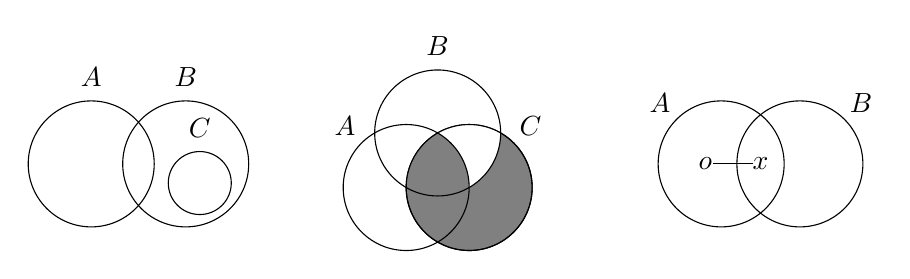
\begin{tikzpicture}
\draw (0,0)     circle (8mm) +(90:11mm) node {$A$};
\draw (0:12mm)  circle (8mm) +(90:11mm) node {$B$};
\draw (-10:14mm) circle (4mm) +(90:7mm) node {$C$};

\begin{scope}[xshift=40mm,yshift=-3mm]
\draw[fill=gray] (0:8mm) circle (8mm);
\begin{scope}
 \clip (60:8mm) circle (8mm);
 \fill[white] (0:8mm) circle (8mm);
 \clip (0,0) circle (8mm);
 \fill[gray] (0:8mm) circle (8mm);
\end{scope}
\draw (0,0)     circle (8mm) +(135:11mm) node {$A$};
\draw (60:8mm) circle (8mm) +(90:11mm) node {$B$};
\draw (0:8mm)  circle (8mm) +(45:11mm) node {$C$};
\end{scope}

\begin{scope}[xshift=85mm]
\draw (-5mm,0) circle (8mm) +(135:11mm) node {$A$};
\draw (5mm,0) circle (8mm)  +(45:11mm) node {$B$};
\node at (-7mm,0) {$o$};
\node at (0,0)    {$x$};
\draw (-6mm,0) to (-1mm,0);
\end{scope}
\end{tikzpicture}
\caption{Euler diagram, Venn diagram, and Peirce's extension to Venn}
\label{fig:eulerandvenn}
\end{figure}

\textcite{Peirce1933} extended Venn diagrams to also express existential
statements and disjunction. He used the symbol $o$ instead of shading to denote
empty sets and the symbol $x$ to represent the existence of an element in a
set. These symbols can be connected by lines that represent disjunctive
statements. Figure~\ref{fig:eulerandvenn} (right) shows a graphical
representing of the statement $A \setminus B = \emptyset \lor A \cup B \neq
\emptyset$ for two sets $A$ and $B$.  Peirce's diagrams were further modified
by \textcite{Shin1995} in two variants that both use Venn's shading instead of
Peirce's symbol $o$. Several extensions and modification to these diagram types
have since been proposed \cite{Howse2008,Dau2009b} and it has been shown that
diagrammatic logic systems can be as complete and as precise as other symbolic
systems for logic sentences and proofs \cite{Hammer1994}. 

Two particular extensions to Peirce/Shin diagrams are spider diagrams and
constraint diagrams, both shown in figure~\ref{fig:spiderdiagram}.
\Term[spider diagram]{Spider diagrams} \cite{Gil1999a}\footnote{In different
context, the term `spider diagram` is also used for other kinds of diagrams,
among them \term{mind maps}.} extend Euler diagram by shading and so called
`spiders' to place lower and upper limits on the number of elements in a set.
Spiders are similar to Peirce's connected $x$ symbols: a spider represents an
element, depicted as a \term{tree} with nodes (shown as dots instead of $x$) in
different zones of the Euler diagram.  Figure~\ref{fig:spiderdiagram} (left)
shows a spider diagram with two spiders.  The first spider indicates that there
is an element which is either in $A$ or in $B$ but not in their intersection.
The shading of $B$ indicates that this element is the only element in $B$. The
second spider indicates that there is another element which is either in $A
\setminus B$ or in $A \cup B$ (being the only element in this intersection) or
neither in $A$ nor $B$. The expressivity of spider diagrams is equivalent to
monadic first order logic with equality.  \Term[constraint diagram]{Constraint
diagrams} \cite{Gil1999b,Gil2001} extend spider diagrams by binary relations
between sets and by explicit universal quantification.
Figure~\ref{fig:spiderdiagram} (right) shows a constraint diagram with two sets
$A$ and $B$ and two disjoint relations $f$ and $g$ ($\forall x \in A,
\tuple{x,y_1} \in f, \tuple{x,y_2} \in g: y_1 \neq y_2$).  Constraint diagrams
have been proposed to replace the \tacro{Object Constraint Language}{OCL}, a
notation for first order predicate logic, that is part of the \acro{UML}
modeling language. While spider diagrams and constraint diagrams have a strong
mathematical background, their actual usability in data modeling is an open
question. Many constraints could also be formulated in a data modeling language
such as \acro{ORM} or in natural language with less rigour and more
readability.

\begin{figure}
\centering
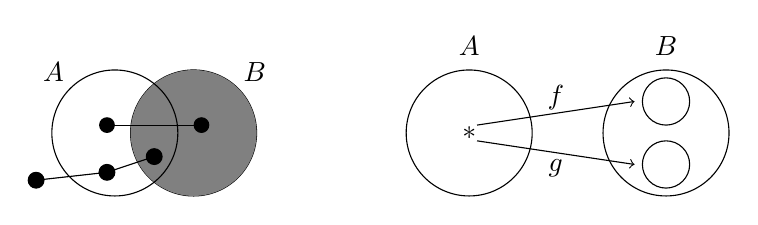
\begin{tikzpicture}
\draw (5mm,0) circle (8mm)  +(45:11mm) node {$B$};
\fill[gray] (5mm,0) circle (8mm);
\draw (-5mm,0) circle (8mm) +(135:11mm) node {$A$};
\fill (-6mm,1mm) circle (1mm);
\fill (+6mm,1mm) circle (1mm);
\draw (-6mm,1mm) to (6mm,1mm);
\draw[fill=black] (0,-3mm) circle (1mm) to (-6mm,-5mm) circle (1mm) to (-15mm,-6mm) circle (1mm);

\begin{scope}[xshift=4cm]
\draw (0,0) node {$*$} circle (8mm) +(90:11mm) node {$A$};
\draw (25mm,0) circle (8mm) +(90:11mm) node {$B$};
\draw (25mm,4mm) circle (3mm);
\draw (25mm,-4mm) circle (3mm);
\draw[->] (1mm,1mm) to node[yshift=2mm] {$f$} (21mm,4mm);
\draw[->] (1mm,-1mm) to node[yshift=-2mm] {$g$} (21mm,-4mm);
\end{scope}
\end{tikzpicture}
\caption{Spider diagram and constraint diagram}
\label{fig:spiderdiagram}
\end{figure}

Another graphical notation for logical sentences, also created by
\textcite{Peirce1933} are \Term[existential graph]{existential graphs}. This
diagram type is divided into three parts.  The first (`Alpha`) corresponds to
\term{propositional logic}, the second (`Beta`) corresponds to
\term{first-order predicate logic}, and the third (`Gamma`) adds elements of
\term{higher-order logic} and \term{modal logic}, among others. The full
system, however, was not finished and existential graphs received little
attention until \textcite{Sowa1976} adopted them to its own \Term{Conceptual
graphs}.  Introductions to conceptual graphs are given by
\cite{Sowa1992,Sowa2008} and \textcite{Dau2009a}. A specification, including the
\tacro{Conceptual Graph Interchange Format}{CGIF} was published as part of
ISO/IEC~24707 (\citeyear{ISO24707:2007}). An example of a conceptual graph from
\textcite{Sowa2008} is shown in example~\ref{ex:cgif} with its notation also
translated to extended \acro{CGIF}.  The graph represents the statement ``if a
cat is on a mat, then it is a happy pet'' -- this interpretation, however,
requires background knowledge in form of a mental model of the real world.
According to \textcite{Sowa2008} the ``\texttt{Attr} relation indicates that
the cat, also called a pet, has an attribute, which is an instance of
happiness'' but what does ``having an attribute, which is an instance of
happines'' mean? One the strict logical level of concetual graphs, there is no
relation between this formal statement and the idea of ``being happy'' and no
knowledge about whether ``being happy'' has a different ontological status than
``being a pet''.\footnote{It is said that cats have no master, so `pet' may be
an attribution just like `happy'.} With their grounding in sets and
relationships, diagrammatic logic systems share strength and weaknesses of
formal logic (section~\ref{sec:logic}): they can be very precise but they
poorly cover non-traditional logic that better fit to descriptions of reality.

A comparision of several diagrammatic logic system for use in \term{artificial
intelligence} is given by \textcite{Sowa1992b}. Diagrammatic logic systems are
very similar to conceptual modeling notations based on entities and
relationships.\footnote{In the first publication on conceptual graphs,
\textcite{Sowa1976} used them to represent the conceptual schemas for database
systems. In later publications he applied them to a wider range of topics from
artificial intelligence and cognitive science.} Both types of diagrams can be
formalized as multi-bipartite graphs or directed multi-hypergraphs from a
graph-theoretic view. 

\begin{example}
\centering
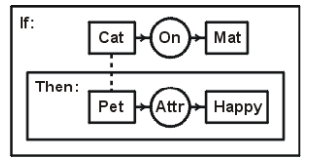
\includegraphics[width=5cm]{img/sowa2008fig7.png}

\verb|[If: [Cat *x] [Mat *y] (On ?x ?y)| \\
\verb|  [Then: [Pet ?x] [Happy *z] (Attr ?x ?z) ]]|

\caption{A conceptual graph in graphical and CGIF notation}
\label{ex:cgif}
\end{example}

\subsubsection{Knowledge structuring diagrams}

The third tradition of conceptual diagrams can best be described as
\Term{knowledge structuring diagrams}. Popular instances include mind maps,
concept maps, topic maps, and spatial hypertext. \textcite{Eppler2006} provides
a comparision of mind maps, concept maps and two additional mapping methods.
As shown by \textcite{Sowa2006}, knowledge structuring diagrams have less
precise semantics than logic diagrams and conceptual modeling notation.  In
data modeling (see figure~\ref{fig:datamodeling} that itself is an example of a
knowledge structuring diagram) they help to find and formulate mental models
without constraints of precise formal logic.

\Term[mind map]{Mind maps} \cite{Buzan1996} arrange topics as possibly colored
bubbles or pictograms with labels in a hierarchical layout around a central
topic. Mind maps are used as tools for brainstorming and note taking, but they
can be hard to read without additional explanation. An example of a mind map is
given in figure~\ref{fig:spatialreltypes} to depict a classfication of spatial
relationship types. In this example topics are drawn as gray bubbles (boxes)
with labels inside and connected by lines. An simple pictogram is shown next to
selected topics (spatial concatenation) for illustration.

\Term[concept]{Concept maps} Concept Maps \cite{Novak2006} arrange labeled
boxes connected by arrows, also starting with a main topic. While mind maps
basically have the graph structure of a labeled \term{tree}, concept maps are
directed labeled graphs. In \Term{spatial hypertext} \cite{Marshall1995} the
basic elements represent documents. Links between documents are shown with
lines and arrows, by inclusion and visual proximity. \Term[topic map]{Topic
Maps} \cite{Pepper2010} are more formally defined, but they neither have
precise semantics such as diagrammatic logic systems. Topic maps are based on
connected topics, similar to concept maps. In addition to elements for topics,
there are associations ($n$-ary relationships between topics with optional
roles) and so called ocurrences. Ocurrences represent information resources
(documents) relevant to particular topics and they may have a \term{datatype}.
As in all conceptual diagrams, elements of topic maps can be labeled by names.
It is possible to treat a topic map as single topic in another topic map
(\term{reification}) but its not clear whether one topic map can refer to itself
in a meaningful way. In contrast to other knowledge diagram types, there are
defined methods to express topic maps in an \acro{XML} based data format and
other precise syntax, and topic maps are standardized in ISO/IEC~13250
(\citeyear{ISO13250}).

% http://www.jfsowa.com/pubs/semnet.htm does not mention Buzan / Mind Maps
% context maps: n-ary links

% good references:
% http://www.springerlink.com/content/2p58r27100r172g6//fulltext.html

% Semantic Networks: directed, labeled graph (Sowa)

% http://www.informationtamers.com/WikIT/index.php?title=Information_map_types

% Sowa, John F. (2000) Knowledge Representation: Logical, Philosophical, and
% Computational Foundations, Brooks/Cole Publishing Co., Pacific Grove, CA,
% Good book on Conceptual graphs: http://www.lirmm.fr/gbkrbook/

% \textcite{Haller2009} present a diagram browsing tool for ``visually structuring
% information objects'': ``"The core top-level relations in CDS e.g. are order
% (before, after, etc.), hierarchy (corresponding to item nesting in iMapping and
% subsuming semantic relations like is a and part of), linking (subsuming
% hyperlinks as well as any other freely specified relation carryingformal
% semantics or not) and annotation (subsuming free-form notes as well as tags and
% types).''

\begin{figure}
\centering
\begin{tikzpicture}
\begin{scope}[mindmap,concept color=gray!20]
\tikzstyle{level 1 concept}+=[font=\sf]
\tikzstyle{level 2 concept}+=[font=\sf]
\tikzstyle{level 3 concept}+=[font=\sf]
\tikzstyle{level 4 concept}+=[font=\sf]
\node[concept,font=\sf,minimum size=20mm,text width=20mm,concept color=gray!40] 
	{spatial\\ relationships}
  child [grow=30]{
  	node[concept,yshift=-10mm]{connections}
	child [grow=150]{ node (lines) [concept]{lines} }
	child [grow=60] { node (arrows) [concept]{arrows} }
	child [grow=-30]{ node (hyperedges) [concept]{hyperedges} }
  }
  child [grow=-100,yshift=5mm]{ 
  	node[concept]{geometric\\ relations}
	child [grow=0]{ node (box) [concept]{box} 
	  child [grow=45]{  node (inclusion) [concept,minimum width=18mm]{inclusion} }
	  child [grow=-15]{ node (intersection) [concept,minimum width=19mm,text width=19mm]{intersection} }
	  child [grow=-80]{ node (concatenation) [concept,text width=22mm,minimum width=22mm,yshift=-5mm]{spatial\\ concatenation} }
	}
  };
\end{scope}

\draw[dotted] (lines.north) ++(-4mm,2mm) to ++(8mm,0mm);
\draw[dotted,->] (arrows.east) ++(1mm,0mm) to ++(8mm,0mm);
\path (hyperedges.north) ++(2mm,3mm) coordinate (x);
\draw[dotted] 
	(x) to +(200:5mm)
	(x) to +(80:6mm)
	(x) to +(-30:5mm);
\draw[dotted] (box.north) ++(-4mm,4mm) circle (5mm and 4mm);
\draw[dotted] (inclusion.north east) ++(3mm,5mm) circle (5mm) ++(1mm,0) circle (3mm);
\draw[dotted] (intersection.north east) ++(3mm,3mm) circle (4mm) ++(4mm,0) circle (4mm);
\draw[dotted] (concatenation.east) ++(4mm,4mm) circle (4mm) ++(8mm,0) circle (4mm);

\end{tikzpicture}
\caption{Mindmap of spatial relationship types in conceptual diagrams}
\label{fig:spatialreltypes}
\end{figure}

\subsubsection{Domain-specific visual notations} Many visual notations exist in
specific domains, such as electrical circuit diagrams, musical notation, and
written singn language \cite{Sutton2002}. Most of them follow some standard
that defines the meaning visual symbols and their aggregations. The common
properties and elements of these domain-specific visual languages, however,
have received little attention so far. \textcite{Tversky2001,Tversky2011}
suggests that visual languages convey meaning rather directly by properties of
the page. Spatial patterns such as proximity, containment, size, and order etc.
help to structure memory, communication and reasoning.

\subsection{Diagram properties}
\label{sec:diagramproperties}

Frameworks to describe and evaluate visual diagram notations are given by
\textcite{Moody2009} by \textcite{Costagliola2004}, and by
\textcite{Bertin2011}.\footnote{First published by \textcite{Bertin1967} in
French.} There are several approaches to describe diagram notations by formal
grammars (see example~\ref{ex:rewritetri} for a simple diagrammatic rewriting
system). The visual symbols of these grammars are constructed by combinations
of visual variables (shape, size, color\ldots) and related to each other by
spatial relationships. The basic relationship types as identified by
\textcite{Costagliola2004} are shown in figure~\ref{fig:spatialreltypes}.
Spatial concatenation can further be divided by direction (above, below, left,
right). A taxonomy of visual variables has been created by
\textcite{Bertin2011}: The basic dimensions are position, size, brightness
value, texture, color, orientation, and shape. Bertin classified these
dimensions according to their suitability to depict quantity, order (ordinal
values), selection (nominal values), and associativity (nominal values with
similarity).  As described by \textcite{Moody2009} these dimensions can be used
as degrees of freedom to encode information, in addition to textual labels as
``non-visual'' elements. All visual elements and dimensions are based on
likenesses and on proximity, at nominal, ordinal, and interval levels
\cite{Tversky2001}. They help to structure memory, communication and reasoning
just like other kinds of patterns. Although the treatment of diagrams as data
requires a first encoding (see appendix~\ref{appendixB}) and although the
domain of non-visual digital data is much more restricted, it is likely that
some visual patterns have counterparts in the domain of non-visual data.


